\subsection{学習方法}
本節において,$\bm{\weightAndBias}$はDNNの全ての重みとバイアスをまとめて表す行ベクトルとする.また,簡潔さを優先して,特別な理由がない限りは重みと呼ぶ.

\subsubsection{損失関数}
損失関数は,DNNによって予測された結果と正解値との間の誤差を求める関数のことであり,扱う問題によって様々である.例えば,回帰問題において用いられる関数の1つに,MAE(Mean Absolute Error)Lossがある.$D$次元の予測対象を$\bm{\outputLower} \in \realSet^{\dimUpper}$,DNNによる予測結果を$\hat{\bm{\outputLower}} \in \realSet^{\dimUpper}$とすると,MAE Lossは
\begin{equation}
    \lossFuncUpper_{\text{MAE}}\lr{\bm{\outputLower}, \hat{\bm{\outputLower}}} = \frac{1}{\dimUpper} \sum_{\dimLower = 1}^{\dimUpper}  \lrAbs{\outputLower_{\dimLower} - \hat{\outputLower}_{\dimLower}}
\end{equation}
で与えられる.また,予測対象が系列長$T$を持った行列$\bm{\outputUpper} \in \realSet^{\timeUpper \times \dimUpper}$の場合,DNNによる予測結果を$\hat{\bm{\outputUpper}} \in \realSet^{\timeUpper \times \dimUpper}$とすると,MAE Lossは
\begin{equation}
    \lossFuncUpper_{\text{MAE}}\lr{\bm{\outputUpper}, \hat{\bm{\outputUpper}}} = \frac{1}{\timeUpper \dimUpper} \sum_{\timeLower = 1}^{\timeUpper} \sum_{\dimLower = 1}^{\dimUpper} \lrAbs{\outputLower_{\timeLower, \dimLower} - \hat{\outputLower}_{\timeLower, \dimLower}}
\end{equation}
で与えられる.

一方,分類問題において用いられる関数の1つに,Cross Entropy Lossがある.$\classUpper$クラス分類の問題について,予測対象を$\bm{\outputLower} \in \lrClosedInterval{0}{1}^{\classUpper}$,DNNによる予測値を$\hat{\bm{\outputLower}} \in \realSet^{\classUpper}$とすると,Cross Entropy Lossは
\begin{equation}
    \lossFuncUpper_{\text{CE}}\lr{\bm{\outputLower}, \hat{\bm{\outputLower}}} = - \sum_{\classLower = 1}^{\classUpper} y_{\classLower} \log \lr{\frac{\exp\lr{\hat{\outputLower}_{c}}}{\sum_{\indexLower = 1}^{C} \exp\lr{\hat{\outputLower}_{c}}}}
\end{equation}
で与えられる.ここで,$\bm{\outputLower}$はクラスに対する確率分布であり,
\begin{equation}
    \sum_{\classLower = 1}^{\classUpper} y_{\classLower} = 1
\end{equation}
を満たす.実際は,正解となるクラスのみを1,それ以外を0としたOne-hotベクトルとされることが多い.また,予測値$\hat{\bm{\outputLower}}$は各クラスに対するスコアを表す値であり,ロジットと呼ばれる.予測対象が行列$\bm{\outputUpper} \in \lrClosedInterval{0}{1}^{\timeUpper \times \classUpper}$の場合,ロジットを$\hat{\bm{\outputUpper}} \in \realSet^{\timeUpper \times \dimUpper}$とすると,Cross Entropy Lossは
\begin{equation}
    \lossFuncUpper_{\text{CE}}\lr{\bm{\outputUpper}, \hat{\bm{\outputUpper}}} = - \frac{1}{\timeUpper} \sum_{\timeLower = 1}^{\timeUpper} \sum_{\classLower = 1}^{\classUpper} y_{\timeLower, \classLower} \log \lr{\frac{\exp\lr{\hat{\outputLower}_{\timeLower, \classLower}}}{\sum_{\indexLower = 1}^{C} \exp\lr{\hat{\outputLower}_{\timeLower, \indexLower}}}}
\end{equation}
で与えられる.

\subsubsection{勾配降下法}
\label{sec3:sec:gradient_descent}
勾配降下法は,損失関数の重みについての勾配を利用して,損失関数の値を最小化するようにDNNを最適化するアルゴリズムである.ここで,学習データセットを$\datasetTrain = \lrc{\lr{\bm{\inputLower}_{\numLower}, \bm{\outputLower}_{\numLower}}}_{\numLower = 1}^{\numUpper}$とする.各$\numLower$に対し,$\bm{\inputLower}_{\numLower} \in \realSet^{\dimUpper_{\text{in}}}$はDNNへの入力, $\bm{\outputLower}_{\numLower} \in \realSet^{\dimUpper_{\text{out}}}$は予測対象を表す.$\dimUpper_{\text{in}}, \dimUpper_{\text{out}}$は入出力の次元である.DNNは$f$とし,予測値を$\hat{\bm{\outputLower}}_{\numLower} = f\lr{\bm{\inputLower}_{\numLower}; \bm{\weightAndBias}}$とする.損失関数は$\lossFuncUpper$とし,$\mathcal{\lossFuncUpper}$を
\begin{equation}
    \mathcal{\lossFuncUpper}\lr{\bm{\weightAndBias}; \mathcal{\indexUpper}} = \frac{1}{\card{\mathcal{\indexUpper}}} \sum_{\indexLower \in \mathcal{\indexUpper}} \lossFuncUpper\lr{\bm{\outputLower}_{\indexLower}, \hat{\bm{\outputLower}}_{\indexLower}} = \frac{1}{\card{\mathcal{\indexUpper}}} \sum_{\indexLower \in \mathcal{\indexUpper}} \lossFuncUpper\lr{\bm{\outputLower}_{\indexLower}, f\lr{\bm{\inputLower}_{\indexLower}; \bm{\weightAndBias}}}
\end{equation}
で定義する.ここで,$\mathcal{\indexUpper} \subset \lrc{1, \ldots, N}$は各サンプルに対するインデックスの部分集合,$\card{\cdot}$は集合の濃度を表す.$\mathcal{\lossFuncUpper}$は学習データ$\lrc{\lr{\bm{\inputLower}_{\indexLower}, \bm{\outputLower}_{\indexLower}}}_{\indexLower \in \mathcal{\indexUpper}} \subset \mathcal{D}_{\text{train}}$に対する損失を,DNNの重み$\bm{\weightAndBias}$の関数として扱うために導入した.上の表記を用いると,DNNの最適化問題は
\begin{equation}
    \min_{\bm{\weightAndBias}} \mathcal{\lossFuncUpper}\lr{\bm{\weightAndBias}; \lrc{1, \ldots, N}}
\end{equation}
と表される.この最適化問題に対し,勾配降下法による重み$\bm{\weightAndBias}$の更新は,
\begin{equation}
    \label{sec3:eq:normal_gradient_descent}
    \bm{\weightAndBias}_{\iter} = \bm{\weightAndBias}_{\iter - 1} - \learningRate \nabla \mathcal{\lossFuncUpper}\lr{\bm{\weightAndBias}_{\iter - 1}; \mathcal{I}_{\iter}}
\end{equation}
で与えられる.ここで,$\iter$は学習におけるイテレーション,$\learningRate$は学習率を表す.

勾配降下法には,3種類の方法がある\cite{zhang2019gradient}.1つ目は,バッチ勾配降下法である.これは,
\begin{equation}
    \bm{\weightAndBias}_{\iter} = \bm{\weightAndBias}_{\iter - 1} - \learningRate \nabla \mathcal{\lossFuncUpper}\lr{\bm{\weightAndBias}_{\iter - 1}; \lrc{1, \ldots, N}}
\end{equation}
で与えられる.すなわち,各イテレーションで学習データ全てを用いる方法である.各サンプルのノイズの影響が低減されることで安定した学習が期待できるが,計算コストが高い.2つ目は,確率的勾配降下法である.これは,ランダムに選択された$n_{\iter} \in \lrc{1, \ldots, N}$に対し,
\begin{equation}
    \bm{\weightAndBias}_{\iter} = \bm{\weightAndBias}_{\iter - 1} - \learningRate \nabla \mathcal{\lossFuncUpper}\lr{\bm{\weightAndBias}_{\iter - 1}; \lrc{n_{\iter}}}
\end{equation}
で与えられる.すなわち,各イテレーションで単一サンプルのみを用いる方法である.計算コストが下がるが,各サンプルのノイズの影響が大きくなることで学習が不安定になる可能性がある.3つ目は,ミニバッチ勾配降下法である.これは,$1 < \card{\mathcal{I}_{\iter}} < N$を満たすランダムに選択された$\mathcal{I}_{\iter} \subsetneq \lrc{1, \ldots, N}$に対し,
\begin{equation}
    \bm{\weightAndBias}_{\iter} = \bm{\weightAndBias}_{\iter - 1} - \learningRate \nabla \mathcal{\lossFuncUpper}\lr{\bm{\weightAndBias}_{\iter - 1}; \mathcal{I}_{\iter}}
\end{equation}
で与えられる.バッチ勾配降下法と確率的勾配降下法の間をとった方法であり,DNNの学習においては一般にミニバッチ勾配降下法が用いられる.ここで,ミニバッチに含まれるサンプルの数をバッチサイズと呼ぶ.

また,確率的勾配降下法やミニバッチ勾配降下法では,サンプルを学習データセットからランダムに非復元抽出する.ここで,毎回のサンプリングされた学習データに対する処理は1イテレーションとカウントし,学習データセットを1度全て使い切ることは1エポックとカウントする.実際には,データセットの総サンプル数$N$に対してバッチサイズを決定することで1エポックあたりの総イテレーション数は決まり,最大エポック数を設定して学習を回すこととなる.

\subsubsection{正則化}
DNNは大量のパラメータにより高い表現力を持つが,その分学習データに過剰に適合し,未知データに対する汎化性能が低いモデルとなる,過学習を引き起こす可能性がある.正則化は,このようなDNNの過学習を防ぐための手段である.以下,具体的な方法を4つ述べる.

1つ目は,L2正則化である.これは,\ref{sec3:sec:gradient_descent}節で定義した$\mathcal{\lossFuncUpper}\lr{\bm{\weightAndBias}; \mathcal{\indexUpper}}$を,
\begin{equation}
    \label{sec3:eq:l2_reg}
    \mathcal{\lossFuncUpper}\lr{\bm{\weightAndBias}; \mathcal{\indexUpper}} = \frac{1}{\card{\mathcal{\indexUpper}}} \sum_{\indexLower \in \mathcal{\indexUpper}} \lossFuncUpper\lr{\bm{\outputLower}_{\indexLower}, f\lr{\bm{\inputLower}_{\indexLower}; \bm{\weightAndBias}}} + \frac{\regConst}{2} \lrTwoNorm{\bm{\weightAndBias}}^{2}
\end{equation}
とすることで与えられる.ここで,$\regConst$は正則化の程度を調整するパラメータである.これより,L2正則化は損失関数の値に$\lrTwoNorm{\bm{\weightAndBias}}^{2}$を加算することで,重み$\bm{\weightAndBias}$のL2ノルムが過大になることを防ぐ方法だと言える.

2つ目は,Weight Decayである.これは,重みの更新式を
\begin{equation}
    \label{sec3:eq:weight_decay}
    \bm{\weightAndBias}_{\iter} = \bm{\weightAndBias}_{\iter - 1} - \learningRate \nabla \mathcal{\lossFuncUpper}\lr{\bm{\weightAndBias}_{\iter - 1}; \mathcal{I}_{\iter}} - \regConst' \bm{\weightAndBias}_{\iter - 1}
\end{equation}
とすることで与えられる.ここで,$\regConst'$は正則化の程度を調整するパラメータである.これより,Weight Decayは重み$\bm{\weightAndBias}$の絶対値が過大になることを防ぐ手法だと言える.

3つ目は,Dropout\cite{srivastava2014dropout}である.Dropoutは,学習時に特徴量の一部を0に落とす手法である.一方,推論時は恒等写像となり,学習時と挙動が変わる.Dropoutへの入力を$\bm{\inputLower} \in \realSet^{\dimUpper}$,特徴量を0に落とす確率を$p$とすると,学習時のDropout出力$\bm{\outputLower}_{\text{train}} \in \realSet^{\dimUpper}$および推論時のDropout出力$\bm{\outputLower}_{\text{infer}} \in \realSet^{\dimUpper}$は,
\begin{align}
    \bm{\outputLower}_{\text{train}} & = \frac{\bm{x} \elemMul \bm{m}}{1 - p} \label{sec3:eq:regularization_dropout_training_output} \\
    \bm{\outputLower}_{\text{infer}} & = \bm{x}
\end{align}
で与えられる.ここで,$D$は特徴量の次元,$\bm{m} \in \lrc{0, 1}^{\dimUpper}$は各成分$m_{\dimLower}$が確率$1 - p$で1,確率$p$で0をとる確率変数である.式\eqref{sec3:eq:regularization_dropout_training_output}より,学習時はDropout出力を$1 / \lr{1 - p}$倍していることがわかる.この理由は,学習時の出力の期待値と推論時の出力を一致させるためである.実際,確率変数$\bm{m}$の従う確率分布上で$\bm{\outputLower}_{\text{train}}$の期待値をとれば,
\begin{align}
    \expectation{\bm{\outputLower}_{\text{train}}} & = \expectation{\frac{\bm{x} \elemMul \bm{m}}{1 - p}}             \\
                                                   & = \frac{\bm{x}}{1 - p} \elemMul \expectation{\bm{m}}             \\
                                                   & = \frac{\bm{x}}{1 - p} \elemMul \lr{1 - p ~ \cdots ~ 1 - p}^\top \\
                                                   & = \bm{x} = \bm{\outputLower}_{\text{infer}}
\end{align}
となる.仮に学習時の挙動のまま推論を行えば,同じ入力を与えても出力は変化するため,複数パターンの出力の期待値を最終出力とすることで,アンサンブルモデルのように汎化性能の向上が期待される.しかし,これは計算コストの増大につながる.Dropoutではこの課題に対して,学習時の出力を$1 / (1 - p)$倍することで,1度の計算でアンサンブルモデルの効果を得られるよう設計されている.これにより,汎化性能を向上させつつ,計算コストが増加しないようになっている.

4つ目は,Early Stoppingである.Early Stoppingは,検証データに対する損失の増加を監視し,設定したエポック数だけ増加し続けた場合に学習を停止する手法である.これにより,学習データに対する過度なフィッティングを防止する.

\subsubsection{最適化手法}
\label{sec3:sec:optimizer}
\ref{sec3:sec:gradient_descent}節において,DNNの重みが勾配降下法によって最適化されることを述べた.ここで,通常の勾配降下法に代わり,近年よく用いられる最適化手法としてAdam\cite{kingma2014adam}がある.Adamの計算過程をアルゴリズム\ref{sec3:algo:adam}に示す.ここで,$\bm{g}_{\iter}$は勾配の1次モーメント,$\bm{m}_{\iter}$が勾配の1次モーメントの指数移動平均,$\bm{v}_{\iter}$が勾配の2次モーメントの指数移動平均である.$\hat{\bm{m}}_{\iter}$および$\hat{\bm{v}}_{\iter}$はそれぞれ,$\bm{m}_{\iter}$および$\bm{v}_{\iter}$の初期値が0であることに起因するバイアスを防ぐための計算を行った結果である.$\optimEmaConst_{1}, \optimEmaConst_{2}$は,指数移動平均の程度を調整するパラメータである.また,9行目のベクトルの平方根および,ベクトルとベクトルの割り算は,各成分ごとに行われる.Adamでは,$\hat{\bm{m}}_{\iter}$を勾配の代わりに用いることで,ミニバッチごとのノイズに対する頑健な学習を可能にする.また,$\hat{\bm{v}}_{\iter}$の平方根で$\hat{\bm{m}}_{\iter}$を割ることによって,勾配の大きさに対するスケーリングを行っている.
\begin{algorithm}
    \caption{Adam}
    \label{sec3:algo:adam}
    \begin{algorithmic}[1]
        \State \textbf{Input:} $\learningRate$, $\optimEmaConst_{1}$, $\optimEmaConst_{2}$, $\regConst$, $\bm{\weightAndBias}_{0}$, $L\lr{\bm{\weightAndBias}}$
        \State $\bm{m}_{0} = 0$, $\bm{v}_{0} = 0$
        \For{$\iter = 1$ to \texttt{...}}
        \State $\bm{g}_{\iter} = \nabla \mathcal{\lossFuncUpper}\lr{\bm{\weightAndBias}_{\iter - 1}; \mathcal{I}_{\iter}} + \regConst \bm{\weightAndBias}_{\iter-1}$
        \State $\bm{m}_{\iter} = \optimEmaConst_{1} \bm{m}_{\iter-1} + \lr{1 - \optimEmaConst_{1}} \bm{g}_{\iter}$
        \State $\bm{v}_{\iter} = \optimEmaConst_{2} \bm{v}_{\iter-1} + \lr{1 - \optimEmaConst_{2}} \bm{g}_{\iter} \elemMul \bm{g}_{\iter}$
        \State $\tilde{\bm{m}}_{\iter} = \bm{m}_{\iter} / \lr{1 - \optimEmaConst_{1}^{\iter}}$
        \State $\tilde{\bm{v}}_{\iter} = \bm{v}_{\iter} / \lr{1 - \optimEmaConst_{2}^{\iter}}$
        \State $\bm{\weightAndBias}_{\iter} = \bm{\weightAndBias}_{\iter-1} - \learningRate \tilde{\bm{m}}_{\iter} / \lr{\sqrt{\tilde{\bm{v}}_{\iter}} + \epsilon}$
        \EndFor
        \State \textbf{Return} $\bm{\weightAndBias}_{\iter}$
    \end{algorithmic}
\end{algorithm}
ここで,Adamでは正則化としてL2正則化を採用したが,Weight Decayを採用した最適化手法としてAdamW\cite{loshchilov2017decoupled}がある.AdamWの計算過程をアルゴリズム\ref{sec3:algo:adamw}に示す.正則化がL2正則化からWeight Decayに変わった点以外は同じである.
\begin{algorithm}
    \caption{AdamW}
    \label{sec3:algo:adamw}
    \begin{algorithmic}[1]
        \State \textbf{Input:} $\learningRate$, $\optimEmaConst_{1}$, $\optimEmaConst_{2}$, $\regConst$, $\bm{\weightAndBias}_{0}$, $L\lr{\bm{\weightAndBias}}$
        \State $\bm{m}_{0} = 0$, $\bm{v}_{0} = 0$
        \For{$\iter = 1$ to \texttt{...}}
        \State $\bm{g}_{\iter} = \nabla \mathcal{\lossFuncUpper}\lr{\bm{\weightAndBias}_{\iter - 1}; \mathcal{I}_{\iter}}$
        \State $\bm{m}_{\iter} = \optimEmaConst_{1} \bm{m}_{\iter - 1} + \lr{1 - \optimEmaConst_{1}} \bm{g}_{\iter}$
        \State $\bm{v}_{\iter} = \optimEmaConst_{2} \bm{v}_{\iter - 1} + \lr{1 - \optimEmaConst_{2}} \bm{g}_{\iter} \elemMul \bm{g}_{\iter}$
        \State $\tilde{\bm{m}}_{\iter} = \bm{m}_{\iter} / \lr{1 - \optimEmaConst_{1}^{\iter}}$
        \State $\tilde{\bm{v}}_{\iter} = \bm{v}_{\iter} / \lr{1 - \optimEmaConst_{2}^{\iter}}$
        \State $\bm{\weightAndBias}_{\iter} = \bm{\weightAndBias}_{\iter - 1} - \learningRate \tilde{\bm{m}}_{\iter} / \lr{\sqrt{\tilde{\bm{v}}_{\iter}} + \epsilon} - \learningRate \regConst \bm{\weightAndBias}$
        \EndFor
        \State \textbf{Return} $\bm{\weightAndBias}_{\iter}$
    \end{algorithmic}
\end{algorithm}

\subsubsection{学習率のスケジューリング}
学習率のスケジューリングは,学習率$\learningRate$の値自体を学習の進行に伴って変更するものである.これは,より安定した学習を促したり,より早く学習を収束させたりするのに役立つ手段である.以下,3つのスケジューラを例として述べる.また,各スケジューラを用いた場合における学習率の遷移を図\ref{sec3:fig:lr_scheduler}に示す.

1つ目は,StepLRSchedulerである.これは,初期学習率を$\learningRate_{0}$として,エポック$\epoch$における学習率$\learningRate_{\epoch}$を
\begin{equation}
    \learningRate_{\epoch} = \learningRate_{0} \gamma^{\left\lfloor \epoch / \epoch_{\text{step}} \right\rfloor}
\end{equation}
で与えるスケジューラである.これは,学習が$\epoch_{\text{step}}$エポック進むごとに学習率を$\gamma$倍することで,学習率を段階的に変化させる.シンプルで分かりやすいが,学習率の変化が不連続的になる.

2つ目は,ExponentialLRSchedulerである.これは,$\learningRate_{\epoch}$を
\begin{equation}
    \learningRate_{\epoch} = \learningRate_{0} \exp \lr{ -\gamma \epoch }
\end{equation}
で与えるスケジューラである.学習が1エポック進むごとに学習率を指数関数的に変化させるため,StepLRSchedulerと比較して変化が連続的である.

3つ目は,Cosine Annealing with Warmupである.これは,$\learningRate_{\epoch}$を
\begin{equation}
    \learningRate_{\epoch} =
    \begin{cases}
        \learningRate_{\text{min}} + \lr{ \frac{\epoch}{\epoch_{\text{warmup}}} } \lr{\learningRate_{\text{max}} - \learningRate_{\text{min}}}                                                                                    & \text{if $\epoch < \epoch_{\text{warmup}}$}   \\
        \learningRate_{\text{min}} + \frac{1}{2} \lr{\learningRate_{\text{max}} - \learningRate_{\text{min}}} \lr{ 1 + \cos \lr{ \frac{\lr{\epoch - \epoch_{\text{warmup}}}\pi}{\epoch_{\text{max}} - \epoch_{\text{warmup}}} } } & \text{if $\epoch \ge \epoch_{\text{warmup}}$}
    \end{cases}
\end{equation}
で与えるスケジューラである.ここで,$\learningRate_{\text{min}}$は最小学習率,$\learningRate_{\text{max}}$は最大学習率,$\epoch_{\text{max}}$は最大エポックである.$\epoch_{\text{warmup}}$は学習率を$\learningRate_{\text{min}}$から$\learningRate_{\text{max}}$まで線形に増加させるのにかけるエポック数を指定するパラメータである.エポック数が$\epoch_{\text{warmup}}$以上となれば,$\cos$関数に従って学習率を減衰させる.Cosine Annealing with Warmupは不安定になりがちな学習初期に学習率が低い状態から開始して,徐々に学習率を大きくすることで解の十分な探索を可能にし,その後再び学習率を小さくすることで学習の収束を促すスケジューラである.

\begin{figure}[bt]
    \centering
    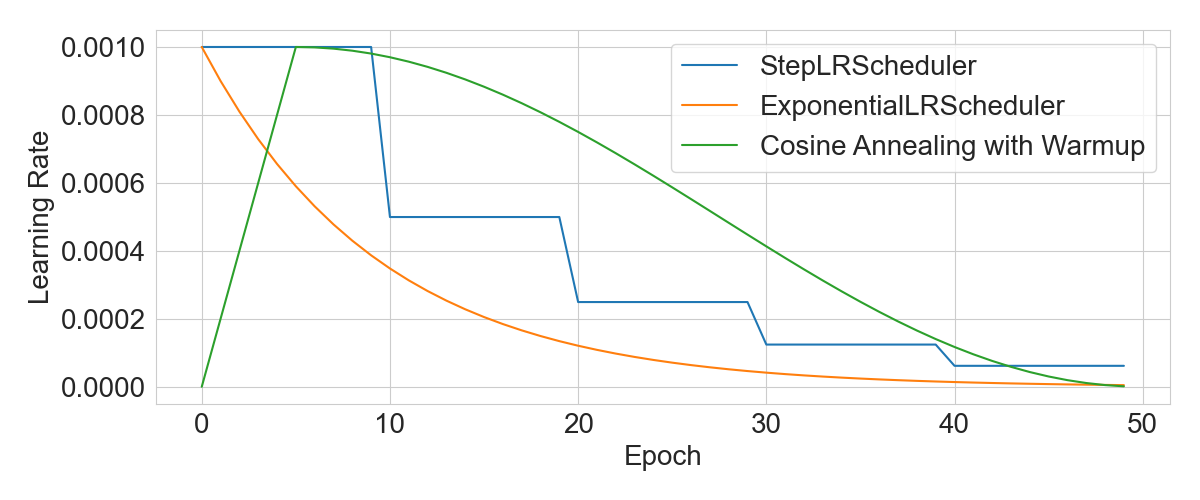
\includegraphics[width=160mm]{./figure/sec3/lr_scheduler.png}
    \caption{スケジューラによる学習率の変化}
    \label{sec3:fig:lr_scheduler}
\end{figure}

\subsubsection{誤差逆伝播法}
\label{sec3:sec:backpropagation}
誤差逆伝播法は,DNNの各重みについての損失関数の勾配を,出力から入力へと遡る方向に計算するアルゴリズムである.ここでは例として,全結合層と活性化関数のみからなる$\numUpper_{\text{layer}}$層のDNNを構築し,ミニバッチ勾配降下法によって最適化する場面を考える\cite{higham2019deep}.また,\ref{sec3:sec:gradient_descent}節で定義した表記を再度用いる.

まず,$\weightLower_{p, q}^{n}$を$n - 1$層目の$p$番目のニューロンから$n$層目の$q$番目のニューロンに割り当てられた重み,$b_{p}^{n}$を$n$層目の$p$番目のニューロンに割り当てられたバイアスとすると,$n$層目の$p$番目のニューロンにおける出力$a_{p}^{n}$は,
\begin{equation}
    \label{sec3:eq:output_before_act}
    a_{p}^{n} = b_{p}^{n} + \sum_{q = 1}^{\dimUpper_{n - 1}} \weightLower_{q, p}^{n} o_{q}^{n - 1}
\end{equation}
で与えられる.ここで,$\dimUpper_{n - 1}$は$n - 1$層目のニューロン数,$o_{q}^{n - 1}$は$n - 1$層目の$q$番目のニューロンにおける出力$a_{q}^{n - 1}$に活性化関数$\phi$を適用した結果を表す.すなわち,
\begin{equation}
    o_{q}^{n - 1} = \phi\lr{a_{q}^{n - 1}}
\end{equation}
である.例外として,各$i \in \mathcal{I}_{\iter}$に対し,$\bm{o}^{0} = \bm{x}_{i}$とする.また,$\dimUpper_{0} = \dimUpper_{\text{in}}, \dimUpper_{N_{\text{layer}}} = \dimUpper_{\text{out}}$とする.ここで,式~\eqref{sec3:eq:output_before_act}に対し,$w_{0, p}^{n} = b_{p}^{n},o_{0}^{n - 1} = 1$とおけば,
\begin{equation}
    \label{sec3:eq:output_before_act_2}
    a_{p}^{n} = b_{p}^{n} + \sum_{q = 1}^{\dimUpper_{n - 1}} w_{q, p}^{n} o_{q}^{n - 1}
    = \sum_{q = 0}^{\dimUpper_{n - 1}} w_{q, p}^{n} o_{q}^{n - 1}
\end{equation}
と整理できる.この時,
\begin{align}
    \pdv{\mathcal{\lossFuncUpper}\lr{\bm{\weightAndBias}; \mathcal{\indexUpper}_{\iter}}}{w_{p, q}^{n}} & = \pdv{w_{p, q}^{n}} \lr{\frac{1}{\card{\mathcal{\indexUpper}_{\iter}}} \sum_{\indexLower \in \mathcal{\indexUpper}_{\iter}} \lossFuncUpper\lr{\bm{\outputLower}_{\indexLower}, f\lr{\bm{\inputLower}_{\indexLower}; \bm{\weightAndBias}}}} \\
                                                                                                        & = \frac{1}{\card{\mathcal{\indexUpper}_{\iter}}} \sum_{\indexLower \in \mathcal{\indexUpper}_{\iter}} \pdv{\lossFuncUpper\lr{\bm{\outputLower}_{\indexLower}, f\lr{\bm{\inputLower}_{\indexLower}; \bm{\weightAndBias}}}}{w_{p, q}^{n}}     \\
                                                                                                        & = \frac{1}{\card{\mathcal{\indexUpper}_{\iter}}} \sum_{\indexLower \in \mathcal{\indexUpper}_{\iter}} \pdv{\lossFuncUpper_{\indexLower}}{w_{p, q}^{n}}
\end{align}
となる.ここで,$\lossFuncUpper\lr{\bm{\outputLower}_{\indexLower}, f\lr{\bm{\inputLower}_{\indexLower}; \bm{\weightAndBias}}} = \lossFuncUpper_{\indexLower}$とおいた.この時,各$n \in \lrc{1, \ldots, N_{\text{layer}}}$に対し,
$\pdv*{\lossFuncUpper_{\indexLower}}{w_{p, q}^{n}}$は式\eqref{sec3:eq:output_before_act_2}を用いて,
\begin{align}
    \pdv{\lossFuncUpper_{\indexLower}}{w_{p, q}^{n}} & = \pdv{\lossFuncUpper_{\indexLower}}{a_{q}^{n}} \pdv{a_{q}^{n}}{w_{p, q}^{n}}                \\
                                                     & = \delta_{q}^{n} \pdv{w_{p, q}^{n}} \lr{\sum_{r = 0}^{D_{n - 1}} w_{r, q}^{n} o_{r}^{n - 1}} \\
                                                     & = \delta_{q}^{n} o_{p}^{n - 1}
\end{align}
となる.ここで,$\pdv*{\lossFuncUpper_{\indexLower}}{a_{q}^{n}} = \delta_{q}^{n}$とおいた.このとき,最終層($n = \numUpper_{\text{layer}}$)の重みの場合,
\begin{align}
    \pdv{L_{\indexLower}}{w_{p, q}^{\numUpper_{\text{layer}}}} & = \delta_{q}^{\numUpper_{\text{layer}}} o_{p}^{\numUpper_{\text{layer}} - 1}                                                                                                                                                      \\
                                                               & = o_{p}^{\numUpper_{\text{layer}} - 1} \pdv{L_{i}}{a_{q}^{\numUpper_{\text{layer}}}}                                                                                                                                              \\
                                                               & = o_{p}^{\numUpper_{\text{layer}} - 1} \pdv{\lossFuncUpper\lr{\bm{\outputLower}_{\indexLower}, f\lr{\bm{\inputLower}_{\indexLower}; \bm{\weightAndBias}}}}{a_{q}^{\numUpper_{\text{layer}}}}                                      \\
                                                               & = o_{p}^{\numUpper_{\text{layer}} - 1} \pdv{\lossFuncUpper\lr{\bm{\outputLower}_{\indexLower}, \phi\lr{\bm{a}^{\numUpper_{\text{layer}}}}}}{a_{q}^{\numUpper_{\text{layer}}}}                                                     \\
                                                               & = o_{p}^{\numUpper_{\text{layer}} - 1} \nabla \lossFuncUpper\lr{\bm{\outputLower}_{\indexLower}, \phi\lr{\bm{a}^{\numUpper_{\text{layer}}}}} \pdv{\phi\lr{\bm{a}^{\numUpper_{\text{layer}}}}}{a_{q}^{\numUpper_{\text{layer}}}}   \\
                                                               & = o_{p}^{\numUpper_{\text{layer}} - 1} \pdv{\lossFuncUpper\lr{\bm{\outputLower}_{\indexLower}, \phi\lr{\bm{a}^{\numUpper_{\text{layer}}}}}}{\phi\lr{a_{q}^{\numUpper_{\text{layer}}}}} \phi'\lr{a_{q}^{\numUpper_{\text{layer}}}}
\end{align}
となる.これは,入力から出力を計算する順伝搬で得られた値のみに依存するから,直ちに計算可能であることがわかる.一方,最終層以外($1 \le n < \numUpper_{\text{layer}}$)の重みの場合,
\begin{align}
    \pdv{L_{\indexLower}}{w_{p, q}^{n}} & = \delta_{q}^{n} o_{p}^{n - 1}                                                                                                            \\
                                        & = o_{p}^{n - 1} \pdv{L_{i}}{a_{q}^{n}}                                                                                                    \\
                                        & = o_{p}^{n - 1} \sum_{r = 0}^{D_{n + 1}} \pdv{L_{\indexLower}}{a_{r}^{n + 1}} \pdv{a_{r}^{n + 1}}{a_{q}^{n}}                              \\
                                        & = o_{p}^{n - 1} \sum_{r = 0}^{D_{n + 1}} \delta_{r}^{n + 1} \pdv{a_{q}^{n}} \lr{\sum_{s = 0}^{D_{n}} w_{s, r}^{n + 1} o_{s}^{n}}          \\
                                        & = o_{p}^{n - 1} \sum_{r = 0}^{D_{n + 1}} \delta_{r}^{n + 1} \pdv{a_{q}^{n}} \lr{\sum_{s = 0}^{D_{n}} w_{s, r}^{n + 1} \phi\lr{a_{s}^{n}}} \\
                                        & = o_{p}^{n - 1} \sum_{r = 0}^{D_{n + 1}} \delta_{r}^{n + 1} w_{q, r}^{n + 1} \phi'\lr{a_{q}^{n}}                                          \\
                                        & = o_{p}^{n - 1} \phi'\lr{a_{q}^{n}} \sum_{r = 0}^{D_{n + 1}} \delta_{r}^{n + 1} w_{q, r}^{n + 1}
\end{align}
となる.これは,順伝搬時には計算されない$\delta_{r}^{n + 1}$に依存しているから,$n + 1$層目についての勾配計算を先に行う必要があることがわかる.従って,最終層のみ直ちに勾配を計算可能であり,それ以外の層は自身の次の層に依存しているから,出力から入力へとDNNを遡る方向に計算する,誤差逆伝播法が効率の良いアルゴリズムだと言える.

\subsubsection{学習の安定化}
DNNの学習は勾配降下法によって行われるが,ここで勾配が大きくなりすぎると重みの更新幅が過剰に大きくなり,学習が不安定になる可能性がある.これに対して,Gradient Clippingが有効である.これは,
\begin{equation}
    \nabla \mathcal{\lossFuncUpper}\lr{\bm{\weightAndBias}; \mathcal{I}} \gets \frac{c}{\max \lrc{\lrTwoNorm{\nabla \mathcal{\lossFuncUpper}\lr{\bm{\weightAndBias}; \mathcal{I}}}, c}} \nabla \mathcal{\lossFuncUpper}\lr{\bm{\weightAndBias}; \mathcal{I}}
\end{equation}
で与えられる.ここで,$c$は勾配のL2ノルムに対する閾値である.$\mathcal{\lossFuncUpper}\lr{\bm{\weightAndBias}; \mathcal{I}}$は\ref{sec3:sec:gradient_descent}節で定義した関数を再度用いた.

また,近年は数億単位のパラメータを持つ大規模なDNNも提案されており,こういった規模間のDNNを構築して学習する場合,それ相応のメモリが必要になる.マシンのスペックに対し,バッチサイズを十分小さくすれば基本的に学習は可能であるが,これは各データのノイズの影響が強くなるため,学習を不安定にする要因となる.これに対し,Gradient Accumulationが有効である.Gradient Accumulationは,小さなバッチサイズで計算した勾配を複数イテレーションに渡って累積し,設定したイテレーション数ごとに重みの更新を行う手法である.累積される勾配を$\bm{g}_{\text{accum}}$とすると,この更新は
\begin{equation}
    \bm{g}_{\text{accum}} \gets \bm{g}_{\text{accum}} + \nabla \mathcal{\lossFuncUpper}\lr{\bm{\weightAndBias}_{\iter - 1}; \mathcal{I}_{\iter}}
\end{equation}
で与えられる.ここで,設定した累積回数を$\numUpper_{\text{accum}}$とすると,重み$\bm{\weightAndBias}$の更新は
\begin{equation}
    \bm{\weightAndBias}_{\iter} = \bm{\weightAndBias}_{\iter - 1} - \frac{\learningRate}{\numUpper_{\text{accum}}} \bm{g}_{\text{accum}}
\end{equation}
で与えられる.$\numUpper_{\text{accum}}$回分の勾配を累積した分,重みを更新する際には$1 / \numUpper_{\text{accum}}$倍して平均をとることで,実質的に$\numUpper_{\text{accum}}$倍のバッチサイズにおける学習が可能になる.また,重み更新後は累積した勾配を0にリセットして,次の$\numUpper_{\text{accum}}$回の累積に備える.
